% autosam.tex
% Annotated sample file for the preparation of LaTeX files
% for the final versions of papers submitted to or accepted for 
% publication in AUTOMATICA.

% See also the Information for Authors.

% Make sure that the zip file that you send contains all the 
% files, including the files for the figures and the bib file.

% Output produced with the elsart style file does not imitate the
% AUTOMATICA style. The style file is generic for all Elsevier
% journals and the output is laid out for easy copy editing. The
% final document is produced from the source file in the
% AUTOMATICA style at Elsevier.

% You may use the style file autart.cls to obtain a two-column 
% document (see below) that more or less imitates the printed 
% Automatica style. This may helpful to improve the formatting 
% of the equations, tables and figures, and also serves to check 
% whether the paper satisfies the length requirements.

% Please note: Authors must not create their own macros.

% For further information regarding the preparation of LaTeX files 
% for Elsevier, please refer to the "Full Instructions to Authors" 
% from Elsevier's anonymous ftp server on ftp.elsevier.nl in the
% directory pub/styles, or from the internet (CTAN sites) on
% ftp.shsu.edu, ftp.dante.de and ftp.tex.ac.uk in the directory
% tex-archive/macros/latex/contrib/supported/elsevier.


%\documentclass{elsart}               % The use of LaTeX2e is preferred.

\documentclass[twocolumn]{autart}    % Enable this line and disable the 
                                     % preceding line to obtain a two-column 
                                     % document whose style resembles the
                                     % printed Automatica style.


\usepackage{graphicx}          % Include this line if your 
                               % document contains figures,
%\usepackage[dvips]{epsfig}    % or this line, depending on which
                               % you prefer.
\usepackage{color}
\usepackage{amssymb}
\usepackage{amsmath}
\setcounter{tocdepth}{3}
\usepackage{graphicx}
\usepackage{tikz}
\usepackage{pgfplots}
\usepackage{framed}
\usepackage{listings}
\usepackage{algorithm,algpseudocode}
\usepackage{epstopdf}
\usepackage{cite}
\usepackage{pifont}
\usepackage{todonotes}
\usetikzlibrary{positioning, automata, shapes.arrows, calc, shapes, arrows}
\usetikzlibrary{patterns}
\usepackage{url}
%\newcommand{\tool}{{\sf DSSynth}\xspace}
\begin{document}
\newcommand\tool{{\sf DSSynth}}
\begin{frontmatter}
%\runtitle{Insert a suggested running title}  % Running title for regular 
                                              % papers but only if the title  
                                              % is over 5 words. Running title 
                                              % is not shown in output.

%\thanksref{footnoteinfo}

\title{Safe and Robust Formal Synthesis of Digital Controllers for Continuous Plants with Transient Performance Specifications} % Title, preferably not more 
                                                % than 10 words.

%\thanks[footnoteinfo]{This paper was not presented at any IFAC 
%meeting. Corresponding author M.~T.~Cicero. Tel. +XXXIX-VI-mmmxxi. 
%Fax +XXXIX-VI-mmmxxv.}

\author[oxford]{Alessandro Abate}\ead{alessandro.abate@cs.ox.ac.uk},
\author[manaus]{Iury Bessa}\ead{iurybessa@ufam.edu.br},
\author[oxford]{Dario Cattaruzza}\ead{dario.cattaruzza@cs.ox.ac.uk},
\author[oxford,manaus]{Lucas Cordeiro}\ead{lucas.cordeiro@cs.ox.ac.uk},
\author[oxford]{Cristina David}\ead{cristina.david@cs.ox.ac.uk},
\author[oxford]{Pascal Kessel}\ead{pascal.kesseli@stx.ox.ac.uk},
\author[oxford]{Daniel Kroening}\ead{kroening@cs.ox.ac.uk},
\author[oxford]{Elizabeth Polgreen}\ead{elizabeth.polgreen@linacre.ox.ac.uk}

\address[oxford]{University of Oxford, UK}
\address[manaus]{Federal University of Amazonas, Brazil}

%\author[Paestum]{Marcus Tullius Cicero}\ead{cicero@senate.ir},    % Add the 
%\author[Rome]{Julius Caesar}\ead{julius@caesar.ir},               % e-mail address 
%\author[Baiae]{Publius Maro Vergilius}\ead{vergilius@culture.ir}  % (ead) as shown

%\address[Paestum]{Buckingham Palace, Paestum}  % Please supply                                              
%\address[Rome]{Senate House, Rome}             % full addresses
%\address[Baiae]{The White House, Baiae}        % here.

          
\begin{keyword}                           % Five to ten keywords,  
Digital Control; A/D converters; Control System Synthesis; Transient Analysis; Safety Analysis; Quantization Errors; Sampling.               % chosen from the IFAC 
\end{keyword}                             % keyword list or with the 
                                          % help of the Automatica 
                                          % keyword wizard

%\keywords{
%State-space dynamical models of physical systems; 
%digital controllers; 
%analogue-to-digital converters; 
%time sampling; 
%quantization; 
%fixed-point arithmetic; 
%CEGIS; 
%safety requirements. 
%}


\begin{abstract}                          % Abstract of not more than 200 words.
\textcolor{red}{We have to write a new abstract.}
\end{abstract}

\end{frontmatter}

\section{Introduction}
\textcolor{red}{We have to write a new introduction as well.} 

%\begin{figure}
%\begin{center}
%\includegraphics[height=4cm]{jcaesar.eps}    % The printed column  
%\caption{Gaius Julius Caesar, 100--44 B.C.}  % width is 8.4 cm.
%\label{fig1}                                 % Size the figures 
%\end{center}                                 % accordingly.
%\end{figure}

% OR

%\begin{figure}
%\begin{center}
%\epsfig{file=jcaesar,width=7cm}
%\caption{Gaius Julius Caesar, 100--44 B.C.}
%\label{fig1}
%\end{center}
%\end{figure}


%\subsection{A subsection}
%Marcus Tullius Cicero, 106--43 B.C. was a Roman statesman, orator, 
%and philosopher.  A major figure in the last years of the Republic, 
%he is best known for his orations against Catiline\footnote{
%This footnote should be very brief.}
%and for his mastery of Latin prose \cite{Heritage:92}. He was a 
%contemporary of Julius Caesar (Fig.~\ref{fig1}).

%-------------------------------
\section{Related Work}
\label{sec:relw}
%-------------------------------

\textbf{CEGIS -}
Program synthesis is the problem of computing correct-by-design programs
from high-level specifications. Algorithms for this problem have made
substantial progress in recent years, for instance~\cite{itzhaky2010simple} 
to inductively synthesize invariants for the generation of desired programs.

Program synthesizers are an ideal fit for the synthesis of digital controllers, since
the semantics of programs capture the effects of finite-precision arithmetic
precisely.  In~\cite{DBLP:conf/cdc/RavanbakhshS15}, the authors use CEGIS
for the synthesis of switching controllers for stabilizing continuous-time
plants with polynomial dynamics.  The work extends to affine systems, but is
limited by the capacity of the state-of-the-art SMT solvers for solving
linear arithmetic.  Since this approach uses switching models instead of
linear dynamics for the digital controller, it avoids problems related to
finite precision arithmetic, but potentially suffers from state-space
explosion.  Moreover, in \cite{DBLP:conf/emsoft/RavanbakhshS16} the same
authors use a CEGIS-based approach for synthesizing continuous-time
switching controllers that guarantee \emph{reach-while-stay} properties of
closed-loop systems, i.e., properties that specify a set of goal states and
safe states (constrained reachability).  This solution is based on
synthesizing control Lyapunov functions for switched systems that yield
switching controllers with a guaranteed minimum dwell time in each mode. 
However, both approaches are unsuitable for the kind of control we seek to
synthesize.

The work in~\cite{hscc-paper} synthesizes stabilizing
controllers for continuous plants given as transfer functions by exploiting
bit-accurate verification of software-implemented digital
controllers~\cite{Bessa16}.  While this work also uses CEGIS,
the approach is restricted to digital controllers for stable closed-loop
systems given as transfer function models: 
this results in  a static check on their coefficients.  
By contrast, in the current paper we consider a state-space representation of the physical system, 
which requires ensuring the specification over actual traces of the model, 
alongside the numerical soundness required by the effects of discretisation and finite-precision errors.   
A state-space model has known advantages over the transfer function
representation~\cite{Franklin15}: it naturally generalizes to multivariate systems
(i.e., with multiple inputs and outputs); 
and it allows synthesis of control systems with guarantees on the internal dynamics, e.g.,
to synthesize controllers that make the closed-loop system \emph{safe}.  Our
work focuses on the \emph{safety} of internal states, which is usually
overlooked in the literature.  Moreover, our work integrates an
abstraction/refinement (CEGAR) step inside the main CEGIS loop.

The tool Pessoa~\cite{mazo2010pessoa} synthesizes correct-by-design embedded
control software in a Matlab toolbox.  It is based on the abstraction of a
physical system to an equivalent finite-state machine and on the computation
of reachability properties thereon. 
Based on this safety specification, \mbox{Pessoa} can synthesize embedded controller
software for a range of properties.  The embedded controller software can be
more complicated than the state-feedback control we synthesize, and the
properties available cover more detail. 
However, relying on state-space discretization \mbox{Pessoa} is likely to incur in scalability limitations. 
Along this research line, \cite{Anta2010,liu16} studies the synthesis of digital controllers for continuous dynamics, 
and \cite{zamani2014} extends the approach to the recent setup of Network Control Systems. 

\textbf{Discretization Effects -}
The classical approach to control synthesis has often disregarded digitalization effects, 
whereas more recently modern techniques have focused on
different aspects of discretization, including delayed
response~\cite{Duggirala2015} and finite word length (FWL) semantics, 
with the goal either to verify (e.g.,~\cite{daes20161}) or to optimize
(e.g.,~\cite{oudjida2014design}) given implementations. 

There are two different problems that arise from FWL semantics.  The first
is the error in the dynamics caused by the inability to represent the exact
state of the physical system, while the second relates to rounding and saturation errors
during computation.  In~\cite{fialho1994stability}, a stability measure
based on the error of the digital dynamics ensures that the deviation
introduced by FWL does not make the digital system unstable.  A~more recent
approach~\cite{DBLP:journals/automatica/WuLCC09} uses $\mu$-calculus to
directly model the digital controller so that the selected parameters are
stable by design.  The analyses in~\cite{DBLP:conf/hybrid/RouxJG15,
DBLP:conf/hybrid/WangGRJF16} rely on an invariant computation on the
discrete system dynamics using Semi-Definite Programming (SDP).  While the
former uses bounded-input and bounded-output (BIBO) properties to determine
stability, the latter uses Lyapunov-based quadratic invariants.  In both
cases, the SDP solver uses floating-point arithmetic and soundness is
checked by bounding the error.  An alternative is~\cite{park2016scalable},
where the verification of given control code is performed against a known
model by extracting an LTI model of the code by symbolic execution:  
to account for rounding errors, an upper bound is introduced in the
verification phase.  The work in \cite{picasso2003stabilization}
introduces invariant sets as a mechanism
to bound the quantization error effect on stabilization as an invariant set
that always converges toward the controllable set.  Similarly,
\cite{liberzon2003hybrid} evaluates the quantization error dynamics
and bounds its trajectory to a known region over a finite time period. 
This technique works for both linear and non-linear systems.

%-------------------------------
\section{Preliminaries}
\label{sec:preliminaries}
%-------------------------------

{\color{blue}[IB:] In my opinion, the subsections \ref{ssec:statefeedbackcontrol}, \ref{ssec:ssrepresentation}, are \ref{ssec:stability} are useless for the Automatica audience. In addition, i guess that all the subsections~\ref{ssec:ssrepresentation}-\ref{ssec:performance} should be erased and a new section about formal specification of transient and stability specifications can be created.}

%-------------------------------
\subsection{Notation} 
\label{ssec:notation}
%-------------------------------



%-------------------------------
\subsection{Counterexample Guided Inductive Synthesis} 
\label{ssec:cegis}
%-------------------------------

In order to synthesize closed-loop digital control systems, we use a program
synthesis engine.  Our program synthesizer implements Counter-Example Guided
Inductive Synthesis (CEGIS)~\cite{DBLP:conf/asplos/Solar-LezamaTBSS06}.  We
start by presenting its general architecture followed by describing the
parts specific to closed-loop control systems.  A high-level view of the
synthesis process is given in Figure~\ref{DSSynth_process}.  Steps $1$ to
$3$ are performed by the user and Steps~A to D are automatically performed
by our tool for Digital Systems Synthesis, named \tool.

CEGIS-based control synthesis requires a formal verifier to check whether a
candidate controller meets the requirements when combined with the plant. 
We use the Digital-System Verifier (DSVerifier)~\cite{IsmailBCFF15} in the
verification module for \tool.  It checks the stability of closed-loop control systems and
considers finite-word length (FWL) effects in the digital controller and
uncertainty parameters in the plant model (plant intervals)~\cite{Bessa16}.   

%
%, which accepts the
%digital controller transfer functions together with the plant model.  For
%any digital controller, implementation details should be provided ({\it
%e.g.}, number of bits, realization, and sample time).

\begin{figure*}[t]
\centering
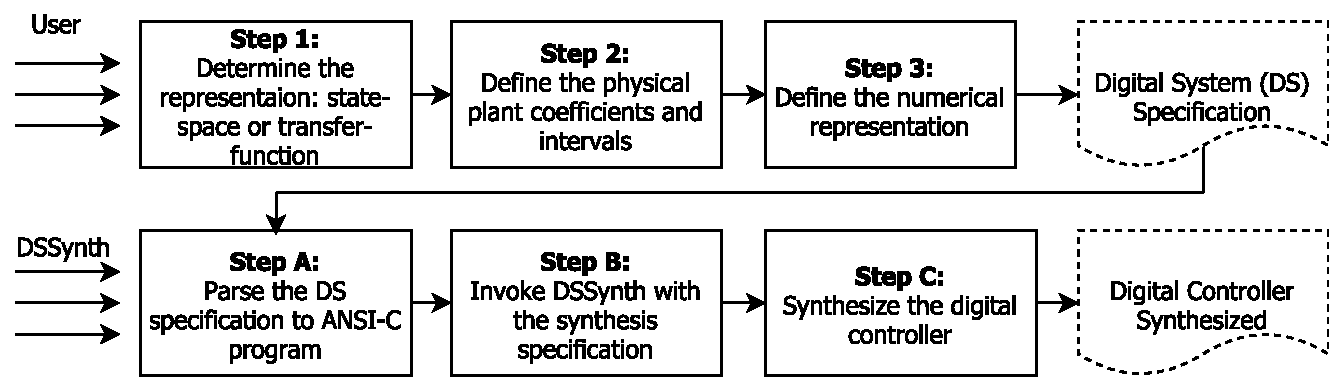
\includegraphics[width=0.9\textwidth]{figures/synthesis-flow.pdf}
\vspace{0.1cm}
\caption{Overview of the synthesis process\label{DSSynth_process}}
\end{figure*}

%In Step $1$, the user provides inputs $G(z)$ and $\Delta{G}(z)$
%%$\%$ ({\it i.e.}, $\Delta{G}(z)$ as a percentage of $G(z)$)
%, which contain the plant model and the
%interval, respectively.  In Step $2$, a digital controller must be designed
%with any preferred method, where $C(z)$ is obtained.  The controller
%numerical representation and realization form are chosen in Steps $3$ and
%$4$, respectively.  In Step $5$, the user finally configures the
%verification parameters ({\it e.g.}, verification time, properties, and BMC
%tool).  After that, DSVerifier verification engine performs an (automatic)
%verification of the desired property $\phi$ ({\it i.e.}, stability).  The
%user steps described in Steps $1$--$5$ result in an ANSI-C code that should
%be used as an input for DSVerifier.

Given a plant model in ANSI-C syntax as input (Steps 1--3), \tool constructs
a non-deterministic model to represent the plant family, i.e., it addresses
plant variations as interval sets (Step~A), and formulates a function
(Step~B) using implementation details provided in Steps~$2$ and $3$ to
calculate the controller parameters to be synthesized (Step~C).  Note that
\tool synthesizes the controller for the desired numerical representation
and realization form.  Finally, \tool builds an intermediate ANSI-C code for
the digital system implementation, which is used as input for the CEGIS
engine (Step~D).

This intermediate ANSI-C code model contains a specification $\phi$ for the
property of interest (i.e., robust stability) and is passed to the
Counterexample-Guided Inductive Synthesis (CEGIS) module of
CBMC~\cite{ClarkeKL04}, where the controller is marked as the input variable
to synthesize.  CEGIS employs an iterative, counterexample-guided refinement
process, which is explained in detail in Section~\ref{synthesizer-general}. 
CEGIS reports a successful synthesis result if it generates a controller
that is safe with respect to~$\phi$.  In particular, the ANSI-C code model
guarantees that a synthesized solution is complete and sound with respect to
the stability property~$\phi$, since it does not depend on system inputs and
outputs.  In the case of stability, the specification~$\phi$ consists of a
number of assumptions on the polynomial coefficients, following Jury's
Criteria, as well as the restrictions on the representation of these
coefficients as discussed in detail in Section~\ref{synthesis-elements}.

%-------------------------------
\subsubsection{CEGIS of digital controllers} 
\label{sssec:cegisdig}
%-------------------------------

%-------------------------------
\subsubsection{Naive approach} 
\label{sssec:naive}
%-------------------------------

\begin{figure}[htb]
{\scriptsize
\centering
%\resizebox{.8\textwidth}{!}
{
 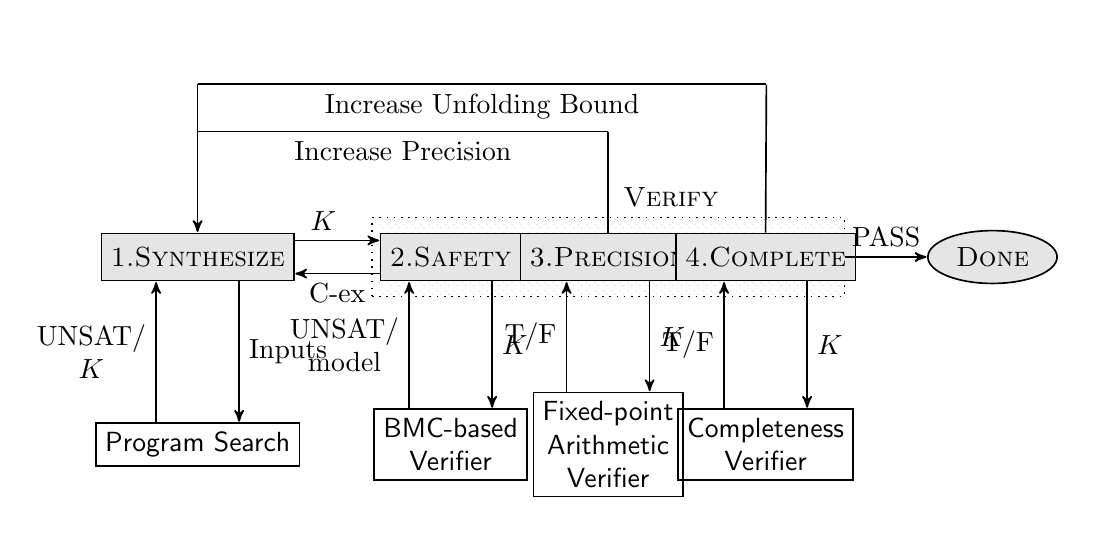
\begin{tikzpicture}[scale=0.3,->,>=stealth',shorten >=.2pt,auto, semithick, initial text=, ampersand replacement=\&,]
  \matrix[nodes={draw, fill=none, shape=rectangle, minimum height=.2cm, minimum width=.2cm, align=center
},
          row sep=.6cm, column sep=.9cm] {
   \coordinate (aux1);
   \& \coordinate (aux2);
   \&;\\
   \coordinate (aux3);
   \& \coordinate (aux4);
   \&;\\
   \coordinate (aux5);
   \& \coordinate (aux6);
   \&;\\
   \node[minimum width=1.5cm, minimum height=0.6cm, fill=gray!20] (synth) {{\sc 1.Synthesize}};
   \&
   complexnode/.pic={ 
     \node[rectangle,draw,dotted,
	minimum width=6cm,
	minimum height=1cm,
        pattern=north west lines, pattern color=gray!20,
	label={\sc ~~~~~~~~~~~~Verify},] (verif) {};
     \node[minimum width=1cm, minimum height=0.6cm, fill=gray!20] (verif1) at ([xshift=-2cm]verif.center) {{\sc 2.Safety}};
     \node[minimum width=1cm, minimum height=0.6cm, fill=gray!20] (verif2) at ([xshift=0cm]verif.center) {{\sc 3.Precision}};
     \node[minimum width=1cm, minimum height=0.6cm, fill=gray!20] (verif3) at ([xshift=2cm]verif.center) {{\sc 4.Complete}};
     %\node[minimum width=1cm, minimum height=0.6cm, fill=gray!20] (verif4) at ([xshift=3.1cm]verif.center) {{\sc 5.Sampling}};
   } 
   \& \node[ellipse, fill=gray!20] (done) {{\sc Done}};\\
   \& \\
   \node[minimum height=0cm] (gp) {\sf Program Search};
   \&
   complexnode/.pic={ 
     \coordinate (aux);
   \node (bmc) at ([xshift=-2cm]aux.center) {\sf BMC-based \\ \sf Verifier};
   \node (fp)  at ([xshift=0cm]aux.center) {\sf Fixed-point \\ \sf Arithmetic\\ \sf Verifier};
   \node (sv)  at ([xshift=2cm]aux.center) {\sf Completeness\\ \sf Verifier};
   %\node (cv)  at ([xshift=3.1cm]aux.center) {\sf Sampling\\Verifier};
   }   
    \\
  };

   \path
    ([yshift=2em]synth.east) edge node[xshift=-0.5em,align=center] {$K$} ([yshift=2em]verif1.west)
    ([yshift=-2em]verif1.west) edge node {C-ex} ([yshift=-2em]synth.east)
    ([xshift=-5em]fp.north) edge node[align=center]  {T/F} ([xshift=-5em]verif2.south)
    ([xshift=-5em]sv.north) edge node[align=center]  {T/F} ([xshift=-5em]verif3.south)
    %([xshift=-5em]cv.north) edge node[align=center]  {T/F} ([xshift=-5em]verif4.south)
    ([xshift=5em]verif1.south) edge node[align=center] {$K$} ([xshift=5em]bmc.north)
    ([xshift=5em]verif2.south) edge node[align=center] {$K$} ([xshift=5em]fp.north)
    ([xshift=5em]verif3.south) edge node[align=center] {$K$} ([xshift=5em]sv.north)
    %([xshift=5em]verif4.south) edge node[align=center] {$K$} ([xshift=5em]cv.north)
    ([xshift=-5em]bmc.north) edge node[align=center]  {UNSAT/\\model} ([xshift=-5em]verif1.south)
    (verif) edge node {PASS} (done)
    ([xshift=5em]synth.south) edge node[align=center] {Inputs} ([xshift=5em]gp.north)
    ([xshift=-5em]gp.north) edge node[align=center] {UNSAT/\\$K$} ([xshift=-5em]synth.south)
    (aux3) edge (synth.north);
   \path[-]
   (verif2.north) edge node[align=center] {} ([xshift=0cm]aux6)
   ([xshift=0cm]aux6) edge node[align=center] {Increase Precision} (aux5)
   (verif3.north) edge node[align=center] {} ([xshift=6.7cm]aux4)
   ([xshift=6.7cm]aux4) edge node[align=center] {Increase Unfolding Bound} (aux3);
   %(verif4.north) edge node[align=center] {} ([xshift=10.5cm]aux2)
   %([xshift=10.5cm]aux2) edge node[align=center] {Increase Sampling Rate} (aux1);

 \end{tikzpicture}
}}
\caption{CEGIS with multi-staged verification}
\label{fig:CEGIS-precision-increment}
\end{figure}

%\subsubsection{Controller synthesis}

An overview of the algorithm for controller synthesis is given in
Fig.~\ref{fig:CEGIS-precision-increment}.  One important observation is that
we verify and synthesize a controller over $k$ time steps.  We~then compute
a completeness threshold $\overline{k}$~\cite{DBLP:conf/vmcai/KroeningS03}
for this controller, and verify correctness for $\overline{k}$ time steps. 
Essentially, $\overline{k}$ is the number of iterations required to
sufficiently unwind the closed-loop state-space system, 
which ensures that the boundaries are not violated for any other $k{>}\overline{k}$.

%\begin{theorem} There exists a finite $\overline{k}$ such that it is
%sufficient to unwind the closed-loop state-space system up to $\overline{k}$
%in order to ensure that $\phi_\mathit{safety}$ holds. 
%\end{theorem}
%
%\begin{proof}
%%
%A stable control system is known to have converging dynamics.  Assume the
%closed-loop matrix eigenvalues are not repeated (which is sensible to do,
%since we select them).  The distance of the trajectory from the reference
%point (origin) decreases over time within subspaces related to real-valued
%eigenvalues; however, this is not the case in general when dealing with
%complex eigenvalues.  Consider the closed-loop matrix that updates the
%states in every discrete time step, and select the eigenvalue $\vartheta$
%with the smallest (non-trivial) imaginary value.  Between every pair of
%consecutive time steps $k\,T_s$ and $(k+1)\,T_s$, the dynamics projected on
%the corresponding eigenspace rotate $\vartheta T_s$ radians.  Thus, taking
%$\overline{k}$ as the ceiling of $\frac{2\pi}{\vartheta T_s}$, after
%$k{\geq}\overline{k}$ steps we have completed a full rotation, which results
%in a point closer to the origin.  The synthesized $\overline{k}$ is the completeness threshold.
%\qed 
%%
%\end{proof}
%
%\medskip

Next, we describe the different phases in Fig.~\ref{fig:CEGIS-precision-increment}
(blocks 1 to 4) in detail.

%\todo{please eventually itemize next}
\begin{enumerate}

\item The inductive synthesis phase ({\sc synthesize}) uses BMC to
compute a candidate solution $K$ that satisfies both the stability criteria
(Sec.~\ref{ssec:stability}) and the safety specification
(Sec.~\ref{ssec:safety}).  To synthesize a controller that satisfies the
stability criteria, we require that a computed polynomial
satisfies Jury's criterion~\cite{fadali}.  The details of this calculation can be found in
the Appendix.


Regarding the second requirement, we synthesize a safe controller by
unfolding the transition system $k$ steps and by picking a controller $K$
and a single initial state, such that the states at each step do not violate
the safety criteria.  That is, we ask the bounded model checker if there
exists a $K$ that is safe for at least one $x_0$ in our set of all possible
initial states.  This is sound if the current $k$ is greater than the completeness
threshold.  We~also assume some precision $\langle I_p,F_p\rangle$ for the
plant and a sampling rate.  The checks that these assumptions hold are
performed by subsequent {\sc verify} stages.

%\begin{algorithm}[]
%\scriptsize
%\begin{algorithmic}[1]
%\Function{$stabilityCheck()$}{}
%  \State computecharPoly($A_d - B_dK$)
%  \State assert(Jury's criteria hold)
  %\State Return $K$
%\EndFunction
%\end{algorithmic}
%\label{alg:stabilitycheck}
%\end{algorithm}


\begin{algorithm}[]
%\scriptsize
\begin{algorithmic}[1]
\Function{$\mathit{safetyCheck}()$}{}
\State assert($ \underline{u}  \leq u \leq \overline{u}$)
 \State set $x_0$ to be a vertex state, e.g., $[\underline{x_0},\underline{x_0}]$	
\For {($c=0;~c < 2^\mathit{Num\_States};~c\mbox{++}$)}
  %\State assert($ \underline{x_0}  \leq x_0 \leq \overline{x_0}$)
	\For{($i=0;~i< k;~i\mbox{++}$)}
		%\State $u = (\langle I_p,F_p\rangle)((\langle I_c,F_c\rangle)K * (\langle I_c,F_c\rangle) x)$
		\State $u = (plant\_typet)((controller\_typet)K * (controller\_typet) x)$
		\State $x = A * x + B * u$
		\State assert($\underline{x} \leq x \leq \overline{x}$ )
  	\EndFor
  	\State set $x_0$ to be a new vertex state
  	\EndFor
  %\State Return $K$
\EndFunction
\end{algorithmic}
\caption{Safety check\label{alg:safetycheck}}
\end{algorithm}

\item The first {\sc verify} stage, {\sc safety}, checks that the candidate
solution $K$, which we synthesized to be safe for at least one initial
state, is safe for \emph{all} possible initial states, i.e., does not reach
an unsafe state within $k$ steps where we assume $k$ to be under the
completeness threshold.  After unfolding the transition system corresponding
to the previously synthesized controller $k$ steps, we check that the safety
specification holds for any initial state. This is shown in Alg.~~\ref{alg:safetycheck}.

\item The second {\sc verify} stage, {\sc precision}, 
 restores soundness with respect to the plant's precision
by using interval arithmetic \cite{moore1966interval} to validate the 
operations performed by the previous stage. 

\item The third {\sc verify} stage, {\sc complete}, checks that the current
$k$ is large enough to ensure safety for any $k'{>}k$.  Here, we compute the
completeness threshold $\overline{k}$ for the current candidate controller $K$ and
check that $k{\geq}\overline{k}$.  This is done according to the argument
given above and illustrated in Fig.~\ref{fig:ct}.

\end{enumerate}

\begin{figure*}[t]
\centering
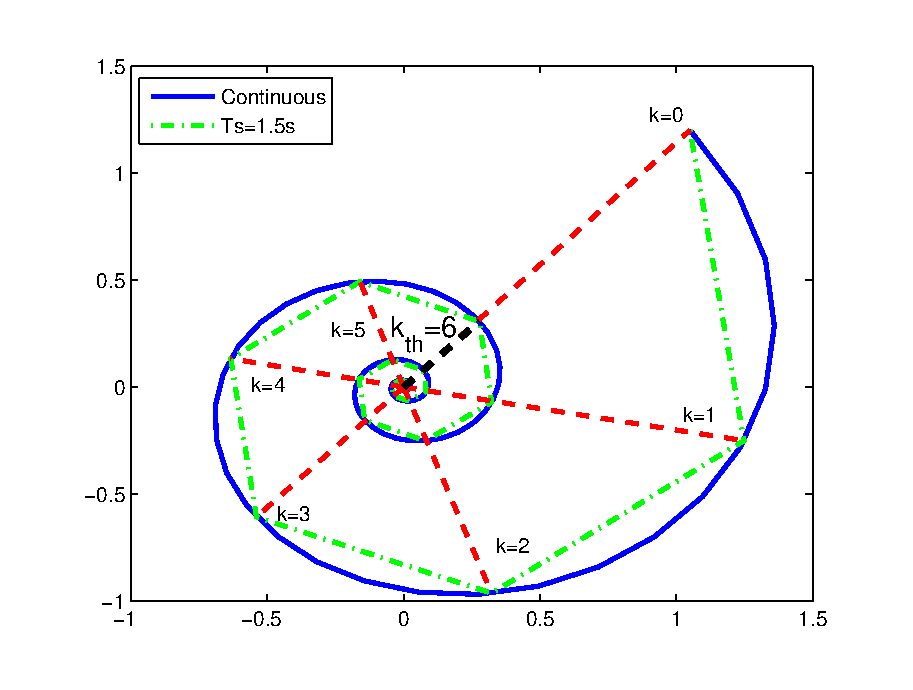
\includegraphics[width=0.6\textwidth]{figures/ct.eps}
\vspace{0.1cm}
\caption{Completeness threshold for multi-staged verification. $T_s$ is the time step for the time discretization of the control matrices.}
\label{fig:ct}
\end{figure*}


Checking that the safety specification holds for any initial state can be 
computationally expensive if the bounds on the
allowed initial states are large. 


%-------------------------------
\subsubsection{Abstraction-based CEGIS} 
\label{sssec:abstraction}
%-------------------------------


  The na\"ive approach described in Sec.~\ref{sec:CEGIS-precision-incrementation}
  %uses a multi-staged verification phase and performs solution generalization based on
%the plant precision, the number of loop unrollings, 
  %and the sampling rate. Essentially, it
  synthesizes a controller for an individual initial state
and input with a bounded time horizon and, subsequently, it generalizes it to all reachable states,
inputs, and time horizons during the verification phase.
Essentially, this approach relies on the symbolic
simulation over a bounded time horizon of individual initial states and inputs that form
part of an uncountable space and tries to generalize it for an
infinite space over an infinite time horizon.

  %% solution over all times by refining the number of witnesses.  
  %% In order to perform the safety check, this approach uses abstract acceleration
  %% \cite{cattaruzza2015unbounded} to compute the controller's set of states. 
  %% \todo{clarify: what is the ``set of states'' of the controller? }
%\end{itemize}

%% The verification of a hybrid continuous/discrete system over an
%% unbounded time, requires the non-deterministic simulation of an
%% infinite set of states, which is undecidable.


%% Our na\"ive approach
%% creates an abstraction of the system by establishing bounds on the
%% error between such a system and a discrete-time/continuous-space
%% model.  This model is still however, quite complex, hard to verify,
%% and many of the states involved are inconsequential to the safety
%% specification.

Conversely, in this section, 
we  find a controller for a continuous initial set of states and set of inputs, 
  over an abstraction of the continuous dynamics \cite{cattaruzza2015unbounded} that conforms to
  witness proofs at specific times. %% It further generalizes the
  Moreover, this approach uses abstraction refinement enabling us to 
  always start with a very simple description regardless of the complexity of the overall
dynamics, and only expand to more complex models when a solution
cannot be found.

  The CEGIS loop for this approach is illustrated in Fig.~\ref{fig:CEGARIS}.

% Now that we have explained the verification process, we may proceed to describe the synthesis procedure, which is illustrated in figure \ref{fig:CEGARIS}.
% Our model, rather than look at a bisimulation \todo{specific notion that has not been formally define - do not use} in discrete time, explores a much higher abstraction, 
% evaluating the unbounded time-continuous space reach tube as a set of inequalities that represent only the safety specification.
% We have also identified 
% the quantization noise as a bounded non-deterministic input.


\begin{enumerate}
\item 
  We start by doing some preprocessing:%%  that 
  %% can be computationally intensive and we don't want it to be part of the CEGIS loop.
% Let us recall the formulas used for single-input and single-output (SISO) systems 
  % in sections \ref{sec:reachable} and \ref{sec:observable}.
  \begin{enumerate}
\item Compute the characteristic polynomial of the matrix $(A_d-B_dK)$ as 
$P_a(z) = z^n+\sum_{i=1}^n{(a_i-k_i)z^{n-i}}$. 
%\blue{[shouldn't there be a b term in the polynomial's coefficients here? No. the polynomial only evaluates the poles]}
%%   A controllable system with quantization will have the following dynamics, where
%% we use underscript ``n'' to denote a noise term,
%% ``cf'' to denote Controllable Canonical Form,
%% $\nu_1$, $\nu_2$ are quantization errors
%% caused by the ADC and DAC conversions, respectively, 
%% and $\nu_3$ is the round-off error.
%% \todo{Why do we use $_t$ here?}
%% %
%% \begin{align}
%% \label{eq:observer_LTI_cf}
%% x_{k+1}=&\mat{A}_{t}x_k+\mat{B}_{t} r_k+\mat{B}_{n} (\nu_1 + \nu_2 + \nu_3)
%% \end{align}
%% \begin{align*}
%% \mat{A}_{t}=&\mat{T}\mat{A}_d\mat{T}^{-1}&
%% \mat{B}_{t}=&\mat{T}\mat{B}_d&
%% \mat{B}_{n}=&[1 \cdots 1]^T&
%% \mat{T}=&\mat{W}_{cf}\mat{W}^{-1}&
%% \end{align*}

%% \begin{align*}
%% \mat{A}_{t}=\mat{T}\mat{A}_d\mat{T}^{-1}=&\left[
%% \begin{array}{ccccc}
%% 0&1&0&\cdots&0\\
%% 0&0&1&\cdots&0\\
%% \vdots&\vdots&\vdots&\ddots&\vdots\\
%% 0&0&0&\cdots&1\\
%% k_n-a_n&k_{n-1}-a_{n-1}&k_{n-2}-a_{n-2}&\cdots&k_1-a_1
%% \end{array}\right]
%% \label{eq:cf_SISO_2}
%% \end{align*}


%% \begin{enumerate}
%% \item Calculate $\mat{T}$ as $\mat{W}_{cf}\mat{W}^{-1}$. %using equations \eqref{eq:rncf}\eqref{eq:rcf}\eqref{eq:to_cf}
%% \item Extract the characteristic polynomial of the above matrix:
%% %
%\begin{align*}
%$P_a = z^n+\sum_{i=1}^p{(a_i-k_i)z^{n-i}}$
%\end{align*}

\item Calculate the noise set $N$ from the quantizer resolutions and estimated round-off errors: %($\frac{q_1}{2},\frac{q_2}{2},q_3$)
%
$$N=\left \{ \nu_1+\nu_2+ \nu_3 : \nu_1 \in \left[-\frac{q_1}{2}\ \ \frac{q_1}{2}\right] 
\wedge \nu_2 \in \left[-\frac{q_2}{2}\ \ \frac{q_2}{2}\right]  \wedge \nu_3 \in \left[-q_3\ \ q_3\right]  \right \}\nonumber$$
%
where  $q_1$ is the error introduced by the truncation in the ADC, $q_2$ is
the error introduced by the DAC and $q_3$ is the maximum truncation and
rounding error in $u_k=-K \cdot \mathcal{F}_{\langle I_c,F_c \rangle}(x_k)$ as
discussed in Section~\ref{sec:numeric_rep}.  More details on how to model
quantization as noise are given in
Appendix~\ref{appendix:quantization-noise}.

\item Calculate a set of initial bounds on $K$, $\phi_\mathit{init}^{K}$,
based on the input constraints %\blue{[how is this practically done?With the equation below]}.  
%
$$(\phi_\mathit{init} \wedge \phi_\mathit{input} \wedge u_k=-K x_k)
\Rightarrow \phi_\mathit{init}^{K}$$
Note that these bounds will be used by the {\sc synthesize} phase to reduce the size of the solution space. 

\end{enumerate}
\item In the {\sc synthesize} phase, we synthesize a candidate controller
%We begin with a minimum set of linear inequalities describing the constraints caused by the input and the initial state during a single iteration, in addition to a stability 
% specification defined by Jury's 
%criteria. %, and try to synthesise a controller that meets these specs.
% For a stabilized closed-loop, which is necessary for our safety property, we need
% these roots to remain within the unit circle, which we verify using Jury's criteria.
% Notice that in our polynomials $c_0=1$ and we only use reals.
% Once we have established convergence, we may examine the 
% safety specification $\phi_\mathit{safety}$.
  $K \in \mathbb{R}\langle I_c,F_c\rangle^n$ that satisfies
  $\phi_\mathit{stability} \wedge \phi_\mathit{safety} \wedge \phi_\mathit{init}^{K}$ by invoking a SAT solver.
%%   We obtain it by solving the SAT formula 
%% $$\mathcal{J}_K=\mathcal{J}\langle I,F \rangle (P_{a-k},\mat{T})\wedge \phi_\mathit{safety}$$ 
%% that satisfies the input constraint and Jury's criteria for 
%% $P_{a-k}=z^n+\sum_{i=1}^n (a_i-k_i) z^{n-i} : k_i \in \mat{K} \wedge \tilde{\mat{K}}=\mat{K}\mat{T}$,
%% where $\mathcal{J}\langle I,F \rangle (P,\mat{T})$ is a program describing Jury's method.
If there is no candidate solution we return UNSAT and exit the loop.
\item Once we have a candidate solution, we perform a safety verification % If this step fails, we find a counterexample iteration and initial state and create a new constraint to refine our abstraction.
  %
  of the 
  %consisting of evaluating the
  progression of the system from $\phi_\mathit{init}$ over time,
$x_{k} \models \phi_\mathit{safety}$. %\blue{why $k+1$ here?}. %% For this purpose we require 
%% an initial set $\phi_\mathit{init}= x_0 \in [\underline{x_0} \ \overline{x_0}]$ 
%% from which the system progresses.
% Obviously, this set $x_0$ 
% must satisfy the specification; otherwise, the system will be unsafe to begin with.
% We accept a specification in the form $\mat{E}\mat{T}x_0<\mat{f}$. 
% The presence of $\mat{T}$ is because this will typically be given in the original 
% state-space.
%% Next, we use abstract acceleration to get a second abstraction that 
  %% encompasses the accelerated continuous reach-tube over an unbounded time.
  In order to compute the progression of point $x_0$ at iteration $k$,
  we accelerate the dynamics of the closed-loop system and obtain:
  %we take the
  %the closed-loop model:
  %$x_{k+1}=\mat{A}_{t}x_k+\mat{B}_{n} (\nu_1 + \nu_2 + \nu_3)$
  %and accelerate it to:
%
\begin{align}
%\label{eq:acc_observer_LTI_cf}
\hspace{-0.1in} x=&(A_d-B_dK)^kx_0
%+\sum_{i=0}^{k-1} \mat{A}_t^i \mat{B}_{t} r_i
+\sum_{i=0}^{k-1} (A_d-B_dK)^i B_{n}(\nu_1+\nu_2+\nu_3) : B_n= [1 \cdots 1]^T
\end{align}
%
As this still requires us to verify the system for every $k$ up to infinity,
we use abstract acceleration again to obtain the reach-tube, i.e., the set
of all reachable states at all times given an initial set
$\phi_\mathit{init}$:
%
\begin{align}
\label{eq:aa_observer_LTI_cf}
\hat{X}^\#
=\mathcal{A} X_0 + \mathcal{B}_{n} N, \quad
X_0 =\left \{x : x \models \phi_\mathit{init} \right\}, 
\end{align}
%
where $\mathcal{A}=\bigcup_{k=1}^\infty (A_d-B_dK)^k,
\mathcal{B}_{n}=\bigcup_{k=1}^\infty \sum_{i=0}^k(A_d-B_dK)^iB_{n}$ are
abstract matrices for the closed-loop system~\cite{cattaruzza2015unbounded},
whereas the set $N$ is non-deterministically chosen.

We next evaluate $\hat{X}^\# \models \phi_\mathit{safety}$.  If the
verification holds we have a solution, and exit the loop.  Otherwise, we
find a counterexample iteration $k$ and corresponding initial point $x_0$
for which the property does not hold, which we use to locally refine the
abstraction.  When the abstraction cannot be further refined, we provide
them to the {\sc abstract} phase.
%
%\todo{we should have a better argument here.}
%\end{enumerate} 
\item If we reach the {\sc abstract} phase, it means that the candidate solution is not valid,
  in which case we must refine the abstraction used by the synthesizer.
\begin{enumerate}
\item Find the constraints that invalidate the property
 as a set of counterexamples for the eigenvalues, which we define as $\phi_\Lambda$. This is a constraint in the spectrum i.e., transfer function) of the closed loop dynamics. 
\item We use $\phi_\Lambda$ to
  further constrain the characteristic polynomial %\blue{[again, check the coefficients of the characteristic polynomial.]I don't find any error} 
$z^n+\sum_{i=1}^n(a_i-k_i)z^{n-i}=\prod_{i=1}^n (z-\lambda_i) : |\lambda_i|<1 \wedge \lambda_i \models \phi_{\Lambda}$. These constraints correspond to specific iterations for which the system may be unsafe.
\item Pass the refined abstraction $\phi(K)$ with the new constraints and the list of iterations $k$ to the {\sc synthesize} phase.
  %, as well as a counterexample plant coefficients ($P_a$) and repeat the loop again. 
\end{enumerate} 
\end{enumerate}

%%-------------------------------
%\subsection{State-space representation of physical systems} 
%\label{ssec:ssrepresentation}
%%-------------------------------
%
%We consider models of physical plants expressed as ordinary differential
%equations (ODEs), which we assume to be controllable and under full state
%information (i.e., we have access to all the model variables):
%%
%\begin{align}
%\label{eq:ode}
%\dot{x}(t) = Ax(t)+ B u(t), \quad x \in \mathbb{R}^{n}, u \in \mathbb{R}^m, \\ \nonumber A \in \mathbb{R}^{n \times n}, B \in \mathbb{R}^{n \times m}, 
%\end{align}
%%
%where $t \in \mathbb R_0^+$, where $A$ and $B$ are matrices that fully
%specify the continuous plant, and with initial states set as $x(0)$.  While
%ideally we intend to work on the continuous-time plant, in this work
%Eq.~\eqref{eq:ode} is soundly discretized in time~\cite{fadali} into
%%
%\begin{align}
%\label{eq:plant}
%x_{k+1} = A_d x_k+ B_d u_k
%\end{align} 
%%
%where $k \in \mathbb N$ and $x_{0}=x(0)$ is the initial state. 
%$A_d$ and $B_d$ denote the matrices that describe the discretized plant dynamics, whereas
%$A$ and $B$ denote the continuous plant dynamics.  
%We synthesize for requirements over this discrete-time domain. 
%Later, we will address the issue of variable quantization, 
%as introduced by the ADC/DAC conversion blocks 
%(\textcolor{red}{we should include a figure that describes the control system model that we tackle}).
%
%
%
%%-------------------------------
%\subsection{Controller synthesis via state feedback}
%\label{ssec:statefeedbackcontrol}
%%-------------------------------
%
%Models \eqref{eq:ode} and \eqref{eq:plant} depend on external non-determinism in the form of input signals $u (t)$ and  $u_k$, respectively. 
%Feedback architectures can be employed to manipulate the properties and behaviors of the continuous process (the plant).   
%We are interested in the synthesis of digital feedback control algorithms, 
%as implemented on Field-Programmable Gate Arrays or Digital Signal Processors. 
%The most basic feedback architecture is the state feedback one, 
%where the control action $u_k$ (notice we work with the discretized signal) is computed by: 
%%
%\begin{equation}
%\label{eq:controlaction}
%u_k = r_{k} - K x_k. 
%\end{equation}
%%
%Here, $K \in \mathbb{R}^{m \times n}$ is a state-feedback gain matrix, 
%and $r_{k}$ is a reference signal (again digital).   
%%
%The closed-loop model then takes the form 
%\begin{align}
%\label{eq:closedloopss}
%x_{k+1} = ( A_d - B_d K ) x_k + B_d r_k.
%\end{align}
%%
%The gain matrix $K$ can be set so that the closed-loop discrete dynamics are
%shaped as desired, for instance according to a specific stability goal or
%around a specific dynamical behavior \cite{astrom1997computer}.  As argued
%later in this work, we will target more complex objectives, such as
%quantitative safety requirements, which are not typical in the digital
%control literature.  Further, we will embrace the digital nature of the
%controller, which manipulates quantized signals as discrete quantities represented with finite precision. 
%
%%-------------------------------
%\subsection{Stability of closed-loop systems}
%\label{ssec:stability}
%%-------------------------------
%
%In this work we employ asymptotic stability in the CEGIS loop,  
%as an objective for guessing controllers that are later proven sound over safety requirements.  
%Asymptotic stability is a property that amounts to convergence of the model executions to an equilibrium point, 
%starting from any states in a neighborhood of the point (see Figure~\ref{fig:ct} for the portrait of a stable execution, converging to the origin).  
%In the case of linear systems as in~\eqref{eq:closedloopss}, 
%considered with a zero reference signal, 
%the equilibrium point of interest is the origin. 
%
%A discrete-time LTI system as \eqref{eq:closedloopss} is asymptotically
%stable if all the roots of its characteristic polynomial (i.e., the
%eigenvalues of the closed-loop matrix $A_d - B_d K$) are inside the unity
%circle of the complex plane, i.e., their absolute values are strictly less than
%one~\cite{astrom1997computer} (this simple sufficient condition can be generalised, 
%however this is not necessary in our work).  
%In this paper, we express this stability specification $\phi_\mathit{stability}$ in terms of a check known as
%\emph{Jury's criterion}~\cite{fadali}: this is an easy algebraic formula to
%select the entries of matrix $K$ so that the closed-loop dynamics are shaped
%as desired.
%
%%-------------------------------
%\subsection{Safety specifications for dynamical systems}
%\label{ssec:safety}
%%-------------------------------
%
%We are not limited to the synthesis of digital stabilizing controllers -- a
%well known task in the literature on digital control systems -- but target
%safety requirements with an overall approach that is sound and automated. 
%More specifically, we require that the closed-loop system
%\eqref{eq:closedloopss} meets given safety specifications.  A safety
%specification gives raise to a requirement on the states of the model, such
%that the feedback controller (namely the choice of the gains matrix~$K$)
%must ensure that the state never violates the requirement.  Note that a
%stable, closed-loop system is not necessarily a safe system: indeed, the
%state values may leave the safe part of the state space while they converge
%to the equilibrium, which is typical in the case of oscillatory dynamics. 
%In~this work, the safety property is expressed as:
%%
%\begin{equation}
%\label{eq:safetyliteral}
%\phi_\mathit{safety}\iff \forall k\ge 0.\, \bigwedge_{i=1}^{n}{\underline{x_{i}} \leq x_{i,k} \leq \overline{x_{i}}},
%\end{equation}
%where $\underline{x_{i}}$ and $\overline{x_{i}}$ are lower and upper bounds
%for the $i$-th coordinate $x_{i}$ of state $x\in \mathbb R^n$ at the $k$-th
%instant, respectively.  This means that the states will always be within an $n$-dimensional hyper-box.
%
%Furthermore, it is practically relevant to consider the 
%constraints $\phi_\mathit{input}$ on the input
%signal $u_{k}$ and $\phi_\mathit{init}$ on the initial states $x_0$,
%which we assume have given bounds:
%$\phi_\mathit{input} = {\forall k.\underline{u} \leq u_{k} \leq \overline{u}} $, 
%$\phi_\mathit{init} = \bigwedge_{i=1}^{n} \underline{x_{i,0}} \leq x_{i,0} \leq \overline{x_{i,0}}.$
%For the former, this means that the control input might saturates in view of
%physical constraints.
%
%%-------------------------------
%\subsection{Performance specifications for dynamical systems}
%\label{ssec:performance}
%%-------------------------------
%
%\textcolor{red}{we should describe here about the performance specifications for dynamical systems.}


%+++++++++++++++++++++++++++++++++++++++++++++++++++++++++++++++++++++++++++++++
\subsection{Numerical representation and soundness} 
\label{sec:numeric_rep}
%+++++++++++++++++++++++++++++++++++++++++++++++++++++++++++++++++++++++++++++++

\textcolor{red}{this section needs to be updated to describe about floating-point arithmetic.}

The models we consider have two sources of error that are due to numerical  
representation.  The first is the numerical error introduced by the
fixed-point numbers employed to model the plant, i.e., to represent the
plant dynamics $A_d$, $B_d$ and $x_k$.  The second is the quantization error
introduced by the digital controller, which performs operations on
fixed-point numbers.  In this section we outline the notation for the
fixed-point representation of numbers, and briefly describe the errors
introduced.  A~formal discussion is in
%Appendix~\ref{appendix:numerical_errors}.

Let $\mathcal{F}_{\langle I,F \rangle}(x)$ denote a real number $x$
represented in a fixed point domain, with $I$ bits representing the integer
part and $F$ bits representing the decimal part.  The smallest number that
can be represented in this domain is $c_m=2^{-F}$.  Any mathematical
operations performed at the precision $\mathcal{F}_{\langle I,F \rangle}(x)$
will introduce errors, for which an upper bound can be
given~\cite{DBLP:conf/arith/BrainTRW15}.

We will use $\mathcal{F}_{\langle I_c,F_c \rangle}(x)$ to denote a real
number $x$ represented at the fixed-point precision of the controller, and
$\mathcal{F}_{\langle I_p,F_p \rangle}(x)$ to denote a real number $x$
represented at the fixed-point precision of the plant model ($I_c$ and $F_c$ are determined by the controller. We pick $I_p$ and $F_p$ for our synthesis such that $I_p \geq I_c$ and $\allowbreak F_p \geq F_c$).  Thus any mathematical operations in our modelled
digital controller will be in the range of $\mathcal{F}_{\langle I_c,F_c
\rangle}$, and all other calculations in our model will be carried out in the range of
$\mathcal{F}_{\langle I_p,F_p \rangle}$.  
The physical plant operates in the
reals, which means our verification phase must also account for the numerical error and quantization errors caused by representing the physical plant at the finite precision $\mathcal{F}_{\langle I_p,F_p \rangle}$.


\subsubsection{Effect on safety specification and stability}

Let us first consider the effect of the quantization errors on safety. 
Within the controller, state values are manipulated at low precision,
alongside the vector multiplication $Kx$.
The inputs are computed using the following equation: 
%
\begin{align*}
u_{k}&=-(\mathcal{F}_{\langle I_c,F_c \rangle}(K)\cdot\mathcal{F}_{\langle I_c,F_c \rangle}(x_{k})). 
\end{align*}

This induces two types of the errors detailed above: first, the truncation
error due to representing $x_k$ as $\mathcal{F}{\langle I_c,F_c
\rangle}(x_{k})$; and second, the rounding error introduced by the
multiplication operation.  We represent these errors as non-deterministic
additive noise.

An additional error is due to the representation of the plant dynamics, namely 
%
\begin{align*}
x_{k+1} &=\mathcal{F}_{\langle I_p,F_p \rangle}(A_d) \mathcal{F}_{\langle I_p,F_p \rangle}(x_{k}) + \mathcal{F}_{\langle I_p,F_p \rangle}(B_d)\mathcal{F}_{\langle I_p,F_p \rangle}(u_{k}).
\end{align*}
We address this error by use of interval
arithmetic~\cite{moore1966interval} in the verification phase.

Previous studies~\cite{gangli1} show that the FWL affects the poles and
zeros positions, degrading the closed-loop dynamics, causing steady-state
errors (see Appendix~\ref{sec:appendix:LTIbackground} for details) and
eventually de-stabilizing the system~\cite{Bessa16}.  However, since in this
paper we require stability only as a precursor to safety, it is sufficient
to check that the (perturbed, noisy) model converges to a neighborhood of
the equilibrium within the safe set (see Appendix~\ref{sec:stab_FWL}).

In the following, we shall disregard these steady-state errors (caused by
FWL effects) when stability is ensured by synthesis, and then verify its
safety accounting for the finite-precision errors.

%-------------------------------
\section{Formal specification of control systems properties} 
\label{sec:specification}
%-------------------------------

%-------------------------------
\subsection{Formal specification of stability} 
\label{ssec:stabspecification}
%-------------------------------


Next, we describe the specific property that we pass to the program
synthesizer as the specification $\sigma$.  There are a number of 
algorithms in our verification engine that can be used for stability analysis~\cite{daes20161, Bessa16}.  
%one based on Schur's decomposition
%and another one based on Jury's criterion~\cite{astrom1997computer}.  
Here we choose Jury's criterion~\cite{astrom1997computer} in view of its efficiency 
and ease of integration within \tool: 
we employ this method to check the stability in the $z$-domain for the
characteristic polynomial $S(z)$ defined in~\eqref{eq:internal_stab_lemma}.
%
% of the matrix $\left( \begin{array}{c} Y \\ U \end{array}\right)$, where $Y(z)$ is the closed-loop system output and U(z) is the controller output. 
%% \red{[unclear: what matrix? We need to clarify the relationship
%% between the char. poly. $S(z)$ and the later quantities $\Delta
%% N_{G}(z), \Delta D_{G}(z)$ and corresponding controller's
%% structure.]}.
%
We~consider the following form for $S(z)$:
%
\begin{equation*}
S(z) = a_0z^N+a_1z^{N-1}+\cdots+a_{N-1}z+a_N=0, a_0\neq0. 
\end{equation*}
%\cdsay{is this for the matrix $\left( \begin{array}{c} Y \\ U \end{array}\right)$?}

% Assuming that $\hat{G}(z) = \frac{\hat{N_G}(z)}{\hat{D_G}(z)}$
% and $\hat{C}(z) = \frac{\hat{N_C}(z)}{\hat{D_C}(z)}$, then:
% $$S(z) = FWL[N_C(z)] \times \hat{N_G}(z) + FWL[D_C(z)] \times \hat{D_G}(z)$$
Next, the following matrix
$M = [m_{ij}]_{(2N-2)\times N}$ is built from $S(z)$ coefficients:
%
$$
M=\left( 
\begin{array}{c}
V^{(0)}\\
V^{(1)}\\
\vdots\\
V^{(N-2)}
\end{array}
\right), 
$$
%
where $V^{(k)} = [v^{(k)}_{ij} ]_{2\times N}$ such that:
%
$$
v_{ij}^{(0)}=\left\{
\begin{array}{ll}
a_{j-1}, & \mbox{if}~i=1\\
v_{(1)(N-j+1)}^{0},&\mbox{if}~i=2
\end{array}
\right.
$$
%
$$
v_{ij}^{(k)}=\left\{
\begin{array}{ll}
0,&\mbox{if}~j>n-k\\
v_{1j}^{(k-1)}-v_{2j}^{(k-1)} . \frac{v_{11}^{(k-1)}}{v_{21}^{(k-1)}}, & \mbox{if}~j\leq n-k ~\mbox{and}~i=1\\
v_{(1)(N-j+1)}^{k},& \mbox{if}~j\leq n-k ~\mbox{and}~i=2\\
\end{array}
\right.
$$
%
and where $k \in \mathbb{Z}$ is such that $0 < k < N - 2$. 
We have that~\cite{astrom1997computer} 
$S(z)$ is the
characteristic polynomial of a stable system if and only if the following four conditions hold:
%\begin{itemize}
%\item 
$R_1: S(1) > 0$;
%\item 
$R_2: (−1)^N S(−1) > 0$;
%\item 
$R_3: |a_0| < a_N$;
%\item 
$R_4: m_{11} > 0 \wedge\allowbreak
      m_{31}>0 \wedge\allowbreak
      m_{51}>0 \wedge \ldots \wedge\allowbreak
      m_{(2N{-}3)(1)}>0$.
%\end{itemize}
%
The stability property is then encoded by a constraint of the form:
$
\phi_\mathit{stability} \equiv (R_1 \wedge R_2 \wedge R_3 \wedge R_4).
$


%-------------------------------
\subsection{Formal specification of safety} 
\label{ssec:safespecification}
%-------------------------------

We are not limited to the synthesis of digital stabilizing controllers -- a
well known task in the literature on digital control systems -- but target
safety requirements with an overall approach that is sound and automated. 
More specifically, we require that the closed-loop system
\eqref{eq:closedloopss} meets given safety specifications.  A safety
specification gives raise to a requirement on the states of the model, such
that the feedback controller (namely the choice of the gains matrix~$K$)
must ensure that the state never violates the requirement.  Note that a
stable, closed-loop system is not necessarily a safe system: indeed, the
state values may leave the safe part of the state space while they converge
to the equilibrium, which is typical in the case of oscillatory dynamics. 
%However, a safe system will always be stable.  
In~this work, the safety property is expressed as:
%
\begin{equation}
\label{eq:safetyliteral}
\phi_\mathit{safety}\iff \forall k\ge 0.\, \bigwedge_{i=1}^{n}{\underline{x_{i}} \leq x_{i,k} \leq \overline{x_{i}}},
\end{equation}
%
%\addtodo{We consider $x_{i}^{-}$ and $x_{i}^{+}$ to be -1 and 1, respectively.}
%
where $\underline{x_{i}}$ and $\overline{x_{i}}$ are lower and upper bounds
for the $i$-th coordinate $x_{i}$ of state $x\in \mathbb R^n$ at the $k$-th
instant, respectively.  This means that the states will always be within an $n$-dimensional hyper-box.

Furthermore, it is practically relevant to consider the 
constraints $\phi_\mathit{input}$ on the input
signal $u_{k}$ and $\phi_\mathit{init}$ on the initial states $x_0$,
which we assume have given bounds:
$\phi_\mathit{input} = {\forall k.\underline{u} \leq u_{k} \leq \overline{u}} $, 
$\phi_\mathit{init} = \bigwedge_{i=1}^{n} \underline{x_{i,0}} \leq x_{i,0} \leq \overline{x_{i,0}}.$
For the former, this means that the control input might saturates in view of
physical constraints.

%-------------------------------
\subsection{Formal specification of transient response} 
\label{ssec:transientspecification}
%-------------------------------

{\color{red} It must be carefully described: it will be an important contribution}

%-------------------------------
\section{CEGIS of digital control system with transient specifications}
\label{sec:method}
%-------------------------------

%-------------------------------
\subsection{Synthesis in frequency domain}
\label{ssec:frequencycegis}
%-------------------------------

%-------------------------------
\subsection{Synthesis of state feedback controllers}
\label{ssec:sscegis}
%-------------------------------

%-------------------------------
\subsection{Synthesis of state observers}
\label{ssec:sobsvcegis}
%-------------------------------

%-------------------------------
\section{Experimental Evaluation}
\label{exp:evaluation}
%-------------------------------


%-------------------------------
\subsection{Description of the benchmarks}
\label{exp:benchmarks}
%-------------------------------


%-------------------------------
\subsection{Objectives}
\label{exp:objectives}
%-------------------------------


%-------------------------------
\subsection{Results}
\label{exp:results}
%-------------------------------

%-------------------------------
\subsection{Threats to validity}
\label{exp:threats-to-validity}
%-------------------------------

%-------------------------------
\section{Conclusions}
\label{sec:conclusions}
%-------------------------------

\textcolor{red}{We need to write a new conclusions about this work.}

%\addtodo{[Move material from \ref{sec:rw} here]}


%\begin{ack}                               % Place acknowledgements
%Partially supported by the Roman Senate.  % here.
%\end{ack}

\bibliographystyle{plain}        % Include this if you use bibtex 
\bibliography{paper}           % and a bib file to produce the 
                                 % bibliography (preferred). The
                                 % correct style is generated by
                                 % Elsevier at the time of printing.

%\begin{thebibliography}{99}     % Otherwise use the  
                                 % thebibliography environment.
                                 % Insert the full references here.
                                 % See a recent issue of Automatica 
                                 % for the style.
%  \bibitem[Heritage, 1992]{Heritage:92}
%     (1992) {\it The American Heritage. 
%     Dictionary of the American Language.}
%     Houghton Mifflin Company.
%  \bibitem[Able, 1956]{Abl:56}
%     B.~C.~Able (1956). Nucleic acid content of macroscope. 
%     {\it Nature 2}, 7--9. 
%  \bibitem[Able {\em et al.}, 1954]{AbTaRu:54}   
%     B.~C. Able, R.~A. Tagg, and M.~Rush (1954).
%     Enzyme-catalyzed cellular transanimations.
%     In A.~F.~Round, editor, 
%     {\it Advances in Enzymology Vol. 2} (125--247). 
%     New York, Academic Press.
%  \bibitem[R.~Keohane, 1958]{Keo:58}
%     R.~Keohane (1958).
%     {\it Power and Interdependence: 
%     World Politics in Transition.}
%     Boston, Little, Brown \& Co.
%  \bibitem[Powers, 1985]{Pow:85}
%     T.~Powers (1985).
%     Is there a way out?
%     {\it Harpers, June 1985}, 35--47.

%\end{thebibliography}

\appendix


%-------------------------------
\section{Stability of Closed-loop Models}
\label{sec:appendix-stability}
%-------------------------------

%-------------------------------
\subsection{Stability of closed-loop models with fixed-point controller error}
\label{sec:stab_FWL}
%-------------------------------

The proof of Jury's criterion~\cite{fadali} relies on the fact that the relationship between states and
next states is defined by $x_{k+1} = (A_d - B_dK) x_k$, all computed
at infinite precision.  When we employ a FWL digital controller, the
operation becomes:
%
\begin{align*}
x_{k+1} &= A_d \cdot x_{k} -(\mathcal{F}_{\langle I_c,F_c \rangle}(K)\cdot\mathcal{F}_{\langle I_c,F_c \rangle}(x_{k})).  \\
x_{k+1} &= (A_d  - B_dK) \cdot x_k + B_dK\delta, 
\end{align*}
%
where $\delta$ is the maximum error that can be introduced by the FWL
controller in one step, i.e., by reading the states values once and
multiplying by $K$ once.  We derive the closed form expression for $x_n$ as
follows:
%
\begin{align*}
x_{1} &= (A_d  - B_dK)x_0 + B_dK\delta \\
x_{2} 
 &=(A_d  - B_dK)^2x_0 + (A_d  - B_dK)B_dK\delta + B_dK\delta \\
x_{n} &= (A_d  - B_dK)^nx_0 + (A_d  - B_dK)^{n-1}B_dK\delta + ... \\  \nonumber & + (A_d  - B_dK)^1B_dK \delta + B_dK\delta \\
  &= (A_d - B_dK)^nx_0 + \sum_{i=0}^{i=n-1}(A_d - B_dK)^iB_dk\delta. 
\end{align*}

The definition of asymptotic stability is that the system converges to a
reference signal, in this case we use no reference signal so an
asymptotically stable system will converge to the origin.  We know that the
original system with an infinite-precision controller is stable, because we
have synthesized it to meet Jury's criterion.  Hence, $(A_d - B_dK)^n x_0$ 
must converge to zero.

The power series of matrices
converges~\cite{horn1990matrix} iff the eigenvalues of the matrix are less
than~1 as follows:
%
%\begin{align*}
$\sum_{i=0}^{\infty}T^i  = (I - T)^{-1}$, 
%\end{align*}
%
where $I$ is the identity matrix and $T$ is a square matrix. Thus, our system will converge to the value 
%
\begin{align*}
0 + (I - A_d + B_dK)^{-1}B_dk\delta \,. 
\end{align*}
%
As a result, if the value $(I - A_d + B_dK)^{-1}B_dk\delta$ is within the
safe space, then the synthesized fixed-point controller results in a safe
closed-loop model.  The convergence to a finite value, however, will not
make it asymptomatically stable.

%+++++++++++++++++++++++++++++++++++++++++++++++++++++++++++++++++++++++++++++++
\section{Errors in LTI models} \label{sec:appendix:LTIbackground}
%+++++++++++++++++++++++++++++++++++++++++++++++++++++++++++++++++++++++++++++++

\subsection{Errors due to numerical representation} \label{appendix:numerical_errors}

We have  used $\mathcal{F}_{\langle I,F \rangle}(x)$ denote a real number
$x$ represented in a fixed point domain, with $I$ bits representing the
integer part and $F$ bits representing the decimal part.  The smallest
number that can be represented in this domain is $c_m=2^{-F}$.  The
following approximation errors will arise in mathematical operations and
representation:
%
\begin{enumerate}

\item {\bf Truncation:} Let $x$ be a real number, and $\mathcal{F}_{\langle
I,F \rangle}(x)$ be the same number represented in a fixed-point domain as
above.  Then $\mathcal{F}_{\langle I,F \rangle}(x) = x-\delta_T$ where the
error $ \delta_T=x\ \%_{c_m}\ \tilde x$, and $\%_{c_m}$ is the modulus
operation performed on the last bit. 
Thus, $\delta_T$ is the truncation error and it will propagate across
operations.
%
\item {\bf Rounding:} The following errors appear in basic operations.  Let
$c_1, c_2$ and $c_3$ be real numbers, and $\delta_{T1}$ and $\delta_{T2}$ be
the truncation errors caused by representing $c_1$ and $c_2$ in the
fixed-point domain as above.
%
\begin{enumerate}
%
\item Addition/Subtraction: these operations only propagate errors coming
from truncation of the operands, namely $\mathcal{F}_{\langle I,F
\rangle}(c_1) \pm \mathcal{F}_{\langle I,F \rangle}(c_2) = c_3 + \delta_3$
with $|\delta_3| \leq |\delta_{T1}| + |\delta_{T2}|$.
%
\item Multiplication: $\mathcal{F}_{\langle I,F \rangle}(c_1) \cdot
\mathcal{F}_{\langle I,F \rangle}(c_2) =  c_3 + \delta_3$ with $|\delta_3|
\leq |\delta_{T1}\cdot\mathcal{F}_{\langle I,F \rangle}(c_2)|\allowbreak +
|\delta_{T2}\cdot\mathcal{F}_{\langle I,F \rangle}(c_1)| + c_m$, where
$c_m=2^{-F}$ as above.
%
\item Division: the operations performed by our controllers in the FWL
domain do not include division.  However, we do use division in computations
at the precision of the plant.  Here the error depends on whether the
divisor is greater or smaller than the dividend:  $\mathcal{F}_{\langle I,F
\rangle}(c_1) / \mathcal{F}_{\langle I,F \rangle}(c_2) = c_3 + \delta_{T3}$
where $\delta_{T3}$ is $(\delta_{T2}\cdot c_1 - \delta_{T1}\cdot
c_2)/(\delta_{T2}^2 - \delta_{T2} c_2)$,
\end{enumerate}

\item {\bf Overflow:}
The maximum size of a real number $x$ that can be represented in a fixed
point domain as $\mathcal{F}_{\langle I,F \rangle}(x)$ is $\pm
(2^{I-1}+1-2^{-F})$.  Numbers outside this range cannot be represented by
the domain.  We check that overflow does not occur.

\end{enumerate}

%+++++++++++++++++++++++++++++++++++++++++++++++++++++++++++++++++++++++++++++++
\subsection{Modeling quantization as noise} \label{appendix:quantization-noise}
%+++++++++++++++++++++++++++++++++++++++++++++++++++++++++++++++++++++++++++++++

During any given ADC conversion, the continuous signal will be sampled in
the real domain and transformed by $\mathcal{F}\langle I_{c},F_{c} \rangle
(x)$ (assuming the ADC discretization is the same as the digital
implementation).  This sampling uses a threshold which is defined by the
less significant bit ($q_{c}=c_{m_c}=2^{-F_c}$) 
of the ADC and some non-linearities of the circuitry.  The overall conversion is
%
$$\mathcal{F}\langle I_{c},F_{c} \rangle(y(t)) = y_k :
y_k \in \left[y(t)-\frac{q_{c}}{2}\ \ \ \ y(t)+\frac{q_{c}}{2}\right] \,.$$
%
If we denote the error in the conversion by $\nu_k=y_k-y(t)$ where $t = nk$,
and $n$ is the sampling time and $k$ the number of steps, then we may define
some bounds for it $\nu_k \in [-\frac{q_{c}}{2}\ \ \frac{q_{c}}{2}]$.

We will assume, for the purposes of this analysis, that the domain of the
ADC is that of the digital controller (i.e, the quantizer includes any
digital gain added in the code).  The process of quantization in the DAC is
similar except that it is calculating $\mathcal{F}\langle I_{dac},F_{dac}
\rangle (\mathcal{F}\langle I_{c},F_{c} \rangle (x)) $.  If these domains
are the same ($I_{c}=I_{dac},\allowbreak F_{c}=F_{dac}$), or if the DAC
resolution in higher than the ADCs, then the DAC quantization error is equal
to zero.  From the above equations we can now define the ADC and DAC
quantization noises ${\nu_1}_k \in [-\frac{q_1}{2}\ \ \frac{q_1}{2}]$ and
${\nu_2}_k \in [-\frac{q_2}{2}\ \ \frac{q_2}{2}]$, where $q_1=q_{c}$ and 
$q_2=q_\mathit{dac}$.  This is illustrated in
Fig.~\ref{ssec:statefeedbackcontrol} where $Q_1$ is the quantizer of the ADC
and $Q_2$ the quantizer for the DAC.  These bounds hold irrespective of
whether the noise is correlated, hence we may use them to over-approximate
the noise effect on the state space progression over time.  The
resulting dynamics are
%
\begin{align*}
%\label{eq:pre_quantization}
{x}_{k+1} = {A}_d{x}_k+{B}_d({u}_k+{{\nu}_2}_k), \quad u_k = -K{x}_{k}+{{\nu}_1}_k, 
\end{align*}
%
which result in the following closed-loop dynamics:
%
\begin{align*}
%\label{eq:quantization}
{x}_{k+1} &= ({A}_d-{B}_d{K}_d) {x}_k+{B}_d{{\nu}_2}_k +{{\nu}_1}_k \,. 
\end{align*}



%\section{A summary of Latin grammar}    % Each appendix must have a short title.
%\section{Some Latin vocabulary}         % Sections and subsections are supported  
                                        % in the appendices.
\end{document}